\documentclass[crop, tikz]{standalone}
\usepackage{tikz}

\usetikzlibrary{calc}

\definecolor{olivegreen}{rgb}{0,0.6,0}

\begin{document}
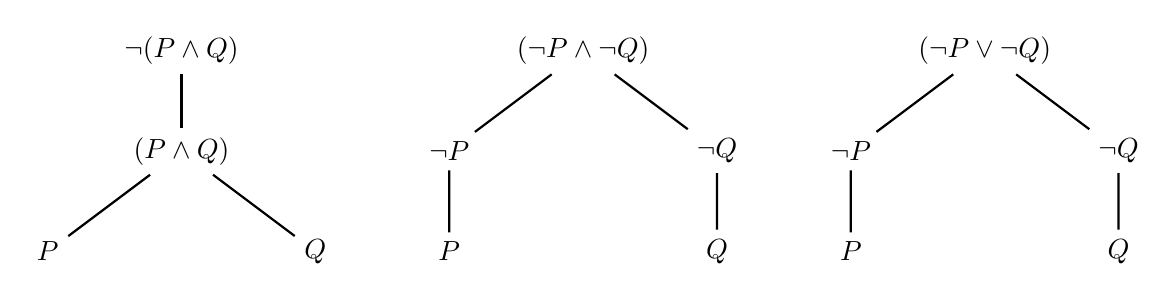
\begin{tikzpicture}[scale=0.85]
	% Axis
%%itikz

        \node at (0,0) (r) { $\neg (P\wedge Q)$};
        \node at (0,-1.5) (n1) { $(P\wedge Q)$};
        \node at (-2,-3) (n2) { $P$};
        \node at (2,-3) (n3) { $Q$};
        
        \path[-,draw,thick] (r) to (n1);
        \path[-,draw,thick] (n1) to (n2);
        \path[-,draw,thick] (n1) to (n3);
        
        \node at (6,0) (r2) { $(\neg P\wedge \neg Q)$};
        \node at (4,-1.5) (n21) { $\neg P$};
        \node at (8,-1.5) (n22) { $\neg Q$};
        \node at (4,-3) (n23) { $P$};
        \node at (8,-3) (n24) { $Q$};
        
        \path[-,draw,thick] (r2) to (n21);
        \path[-,draw,thick] (r2) to (n22);
        \path[-,draw,thick] (n21) to (n23);
        \path[-,draw,thick] (n22) to (n24);

        \node at (12,0) (r3) { $(\neg P\vee \neg Q)$};
        \node at (10,-1.5) (n31) { $\neg P$};
        \node at (14,-1.5) (n32) { $\neg Q$};
        \node at (10,-3) (n33) { $P$};
        \node at (14,-3) (n34) { $Q$};
        
        \path[-,draw,thick] (r3) to (n31);
        \path[-,draw,thick] (r3) to (n32);
        \path[-,draw,thick] (n31) to (n33);
        \path[-,draw,thick] (n32) to (n34);


        
\end{tikzpicture}
\end{document}
